\chapter{PROBLEM IDENTIFICATION AND MOTIVATION}

\section{Introduction}
\label{sec:ch2-introduction}

This chapter grounds the project in the existing literature and formalizes its
requirements. We cover the core concepts behind \ac{LLM}s, fine-tuning for domain
adaptation, the \ac{RAG} paradigm, and the challenges of on-premises deployment.
A comparative study of existing legal \ac{AI} solutions confirms the gap our work
addresses, and we close by defining the functional and non-functional requirements
that will guide the system design.

\section{Large Language Models}
\label{sec:llm-overview}

\subsection{Defining Large Language Models}

A \ac{LLM} can be broadly understood as a deep neural network trained on
massive volumes of textual data with the objective of modeling the statistical
structure of natural language. Unlike earlier \ac{NLP} systems that relied on
hand-crafted rules or shallow pattern matching, \ac{LLM}s learn rich internal
representations of language through exposure to billions of tokens drawn from
diverse sources such as books, web pages, and scientific articles
\cite{brown2020gpt3}. The resulting models are capable of generating coherent
text, answering questions, summarizing documents, and performing a wide range
of language tasks without being explicitly programmed for any of them.

What distinguishes a \ac{LLM} from earlier language models is primarily
its scale, both in terms of parameter count (often ranging from several
billion to hundreds of billions) and the volume of training data consumed.
This scale enables emergent capabilities: behaviors that do not appear in
smaller models but arise once the model reaches a sufficient size, such as
in-context learning and multi-step reasoning \cite{brown2020gpt3}.

\subsection{The Transformer Architecture}

The architecture underpinning virtually all modern \ac{LLM}s is the
Transformer, introduced by Vaswani et al. in 2017 \cite{vaswani2017attention}.
Before its arrival, sequence modeling tasks in \ac{NLP} were dominated by
recurrent neural networks, which processed tokens one at a time in sequential
order. This sequential nature created a bottleneck: long-range dependencies
between distant words were difficult to capture, and training could not be
effectively parallelized across hardware.

The Transformer resolved both limitations through a mechanism called
\textbf{self-attention}. Rather than reading a sequence token by token,
the self-attention mechanism allows every token in a sequence to directly
attend to every other token, computing a weighted representation that
captures contextual relationships regardless of distance. This parallel
computation of attention across all positions makes the Transformer
significantly faster to train on modern \ac{GPU} hardware and far more
effective at modeling long-range dependencies \cite{vaswani2017attention}.

A standard Transformer consists of two main components: an \textbf{encoder},
which reads and encodes the input sequence into a set of continuous
representations, and a \textbf{decoder}, which generates an output sequence
one token at a time by attending to both the encoded input and its own
previously generated tokens. Different model families use different
subsets of this architecture:

\begin{itemize}
    \item \textbf{Encoder-only models} (e.g., \ac{BERT}) focus on
    understanding and classifying input text by building bidirectional
    contextual representations \cite{devlin2019bert}.

    \item \textbf{Decoder-only models} (e.g., \ac{GPT}) generate text
    autoregressively, predicting the next token based on all preceding
    tokens, and form the basis of most modern conversational \ac{LLM}s
    \cite{brown2020gpt3}.

    \item \textbf{Encoder-decoder models} (e.g., T5) combine both
    components and are commonly used for tasks that involve transforming
    one sequence into another, such as translation or summarization.
\end{itemize}

\begin{figure}[H]
\centering
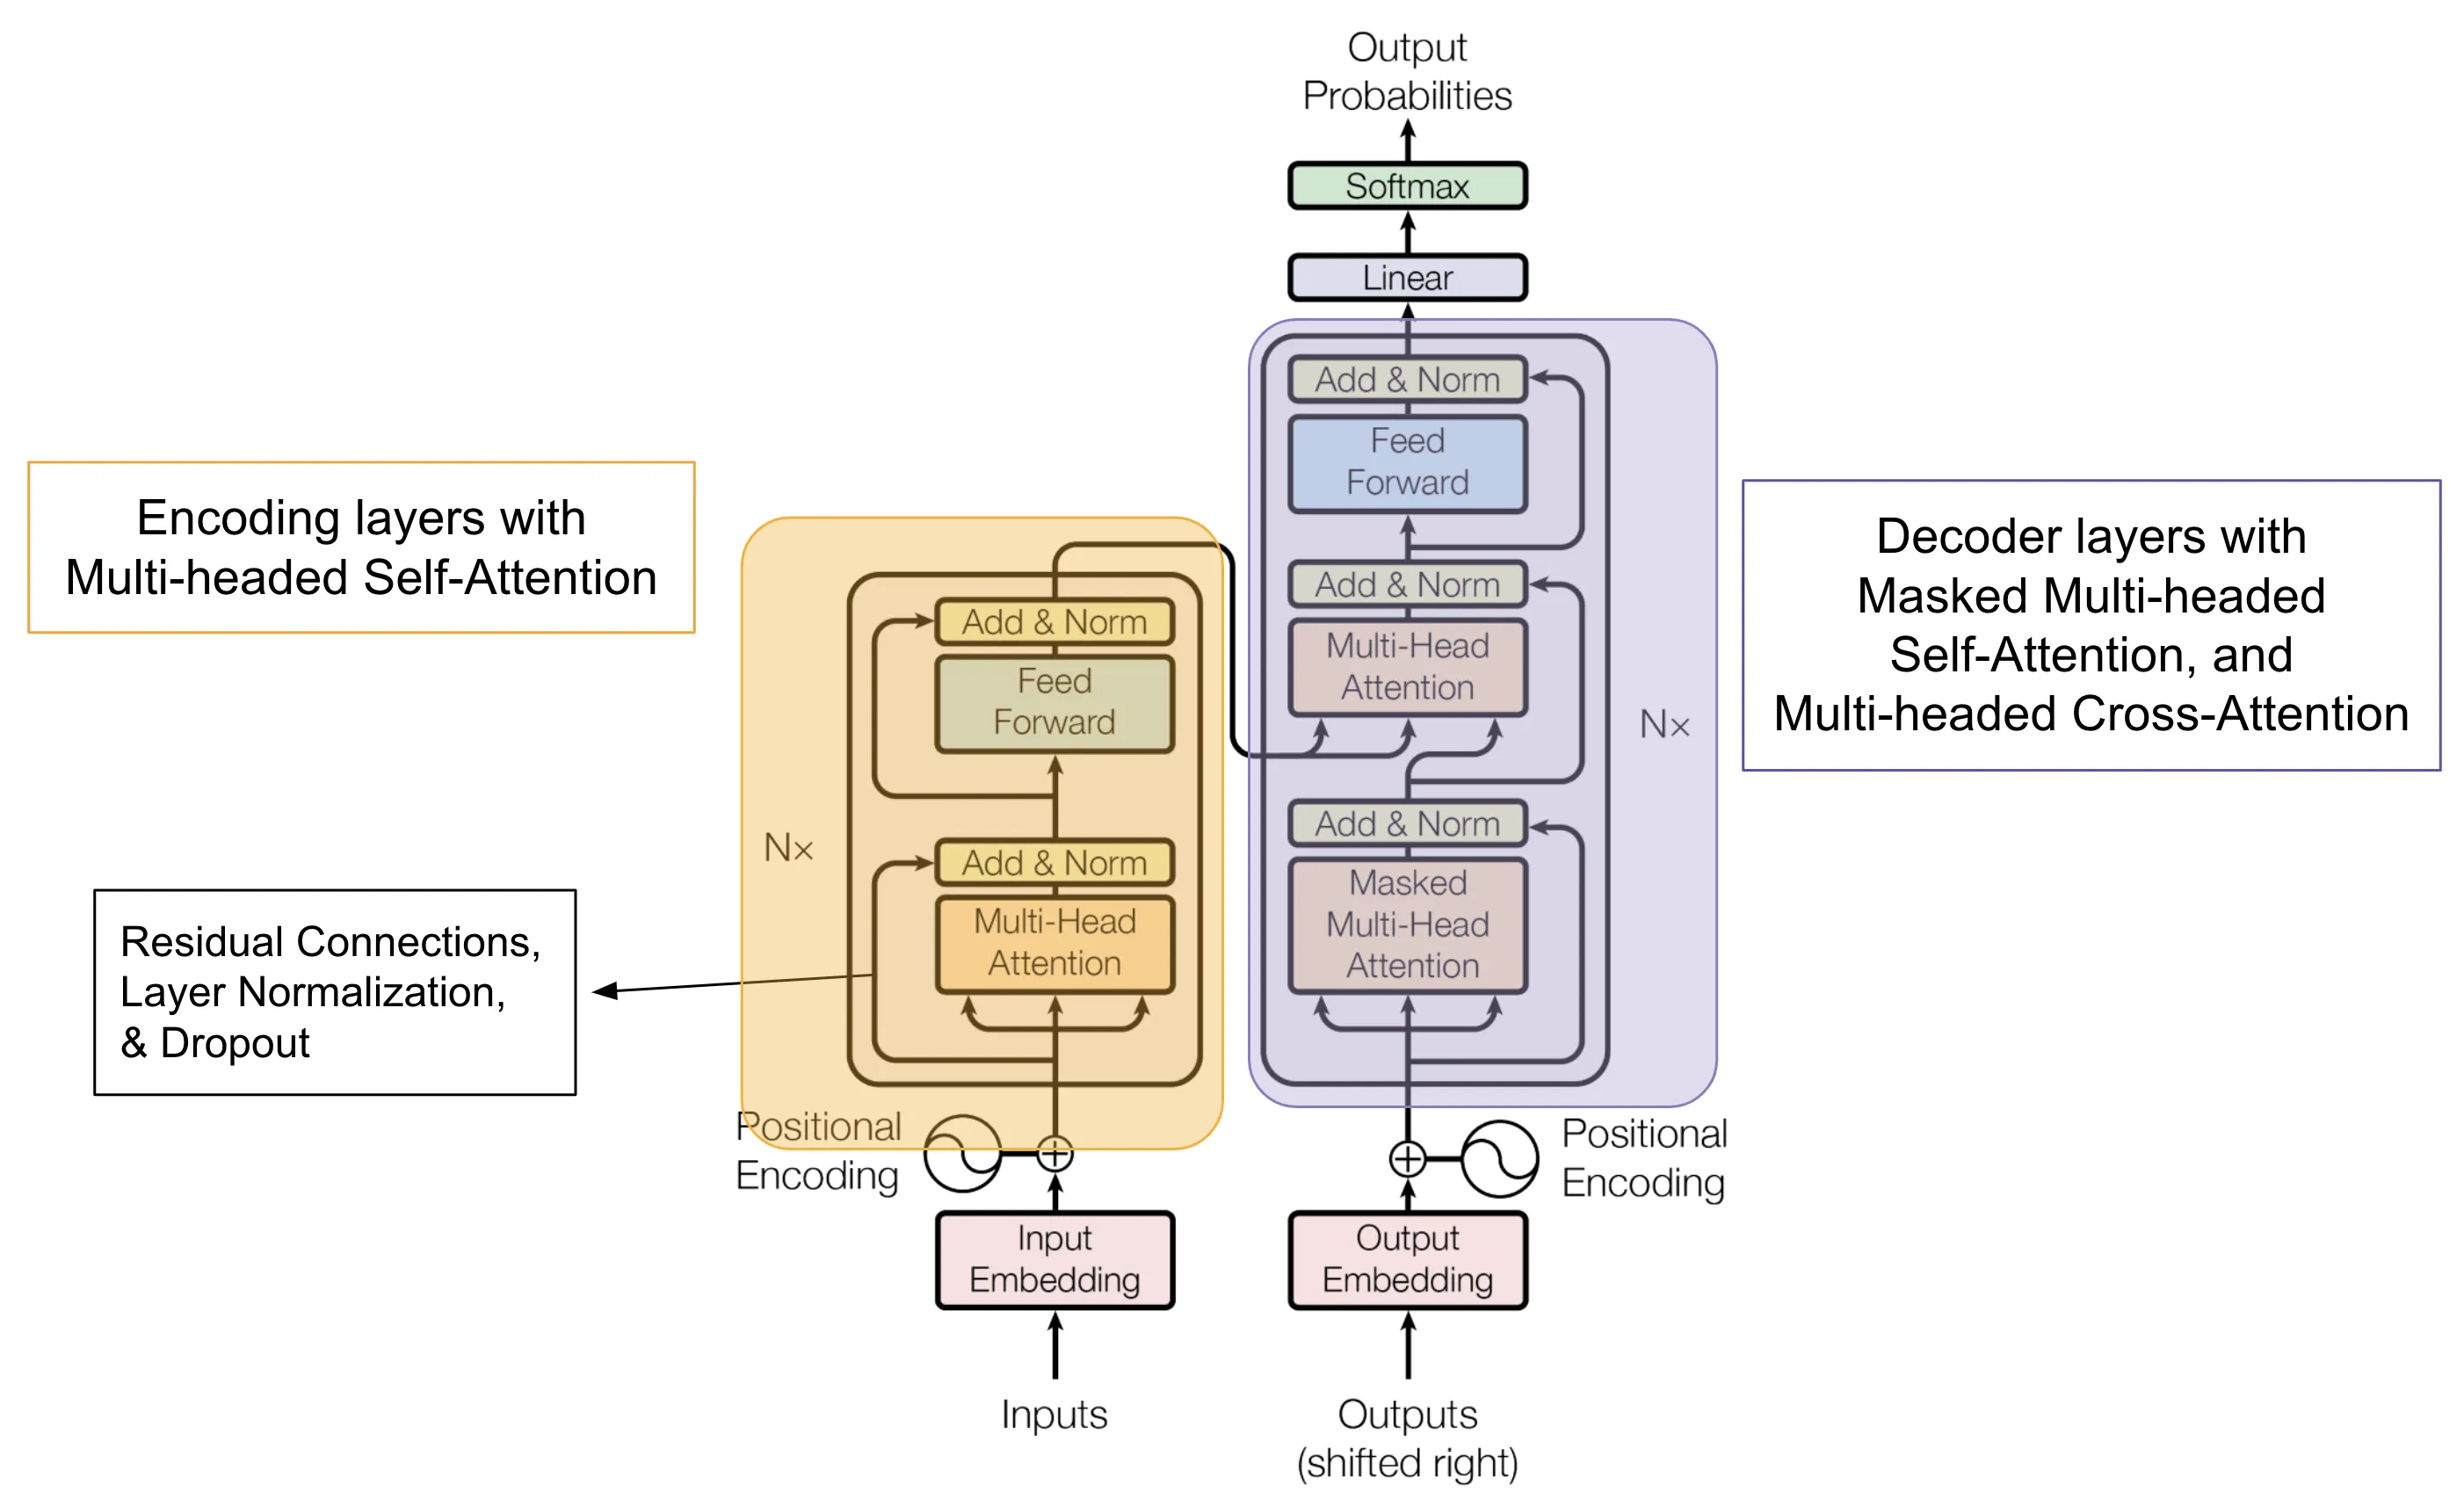
\includegraphics[width=0.8\textwidth]{figures/Annotated-Transformers-Architecture.png}
\caption{The Transformer Architecture \cite{aiml2024transformer}}
\label{fig:transformer}
\end{figure}

\subsection{Pre-Training and Transfer Learning}

The power of \ac{LLM}s stems largely from a two-stage training paradigm.
In the first stage, called \textbf{pre-training}, the model is exposed to
an enormous corpus of unlabeled text and learns to predict the next word
in a sequence (for decoder-only models) or to reconstruct masked words
(for encoder-only models). This unsupervised process forces the model to
internalize grammar, factual knowledge, reasoning patterns, and even
stylistic conventions present in the training data \cite{devlin2019bert}.

The second stage, called \textbf{fine-tuning} or \textbf{transfer learning},
adapts the pre-trained model to a specific downstream task or domain by
continuing training on a smaller, task-specific dataset. Because the model
has already acquired broad linguistic knowledge during pre-training, fine-tuning
requires comparatively little data and computation to achieve strong
performance on the target task. This paradigm has become the standard
approach in modern \ac{NLP}, enabling practitioners to leverage the general
capabilities of large pre-trained models while specializing them for
particular applications \cite{brown2020gpt3}.

\subsection{Key Model Families}

The landscape of open-weight and proprietary \ac{LLM}s has expanded rapidly
in recent years. Several model families are particularly relevant to our project.

\textbf{GPT (OpenAI).} The \ac{GPT} series pioneered the decoder-only
autoregressive approach to language modeling. GPT-3, with 175 billion
parameters, demonstrated that scaling model size and training data could
unlock powerful few-shot learning capabilities. GPT-4 and GPT-4.1
extended these capabilities further with multimodal understanding and
improved instruction following \cite{brown2020gpt3}.

\begin{figure}[H]
\centering
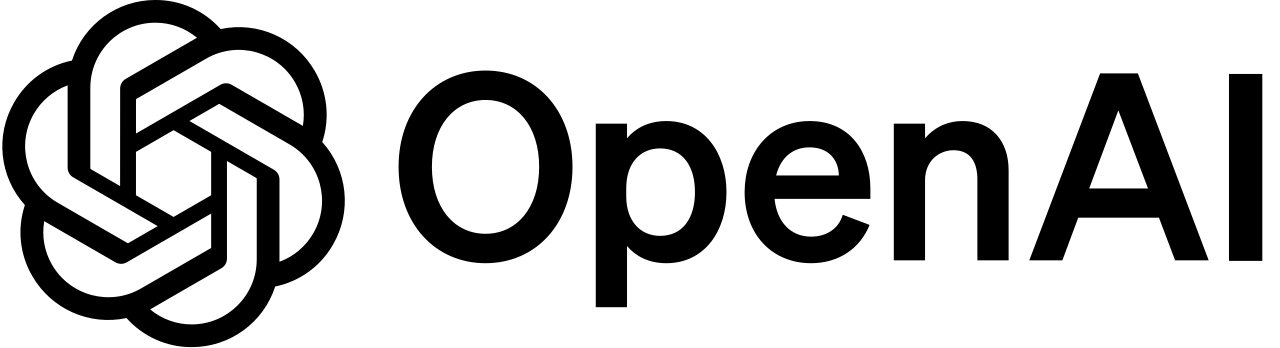
\includegraphics[width=0.2\textwidth]{figures/openai_logo.png}
\caption{GPT - OpenAI \cite{brown2020gpt3}}
\label{fig:openai-logo}
\end{figure}

\textbf{LLaMA (Meta).} The LLaMA family, introduced by Meta,
was designed to achieve strong performance at smaller scales by training
on more data per parameter than previous approaches. LLaMA models range
from 7 billion to 70 billion parameters and have become a popular
foundation for community-driven fine-tuning and adaptation
\cite{touvron2023llama}.

\begin{figure}[H]
\centering

\includegraphics[width=0.2\textwidth]{figures/llama_logo.png}
\caption{LLaMA - Meta \cite{touvron2023llama}}
\label{fig:llama-logo}
\end{figure}

\textbf{Qwen (Alibaba Cloud).} The Qwen family, developed by
Alibaba Cloud, covers a wide range of model sizes from 0.5 billion to
over 70 billion parameters. Qwen models stand out for their strong
multilingual capabilities, with particular emphasis on Arabic and
other non-Latin scripts, making them well suited for applications
that span multiple languages and writing systems \cite{qwen2025qwen25}.

\begin{figure}[H]
\centering

\includegraphics[width=0.2\textwidth]{figures/qwen_logo.jpg}
\caption{Qwen - Alibaba Cloud \cite{qwen2025qwen25}}
\label{fig:qwen-logo}
\end{figure}

\textbf{Gemma (Google).} The Gemma family represents Google's
contribution to the open-weight model ecosystem. Built on the same
research foundations as the Gemini series, Gemma models are available
in compact sizes (2B and 7B parameters) designed for efficient
deployment, making them particularly attractive for on-premises
scenarios with limited hardware resources \cite{gemma2024google}.

\begin{figure}[H]
\centering

\includegraphics[width=0.2\textwidth]{figures/gemma_logo.png}
\caption{Gemma - Google \cite{gemma2024google}}
\label{fig:gemma-logo}
\end{figure}

\section{Fine-Tuning Techniques for Domain Adaptation}
\label{sec:finetuning}

While pre-trained \ac{LLM}s possess broad linguistic competence, they
often lack the specialized vocabulary, reasoning patterns, and domain-specific
knowledge required for high-stakes applications such as legal analysis. Domain
adaptation through fine-tuning addresses this gap by continuing the model's
training on a curated corpus of domain-specific data, allowing it to internalize
the particular conventions, terminology, and logic of the target field.

\subsection{Full Fine-Tuning}

The most straightforward approach to domain adaptation is \textbf{full fine-tuning},
in which all parameters of the pre-trained model are updated using the domain-specific
dataset. During this process, the model's weights are adjusted through standard
backpropagation and gradient descent, allowing every layer of the network to
adapt to the new data distribution.

Full fine-tuning typically produces the highest quality adaptation, as the entire
model capacity is available to learn domain-specific patterns. However, it comes
with significant practical drawbacks: it requires storing and updating a complete
copy of all model parameters, which translates to very high \ac{GPU} memory
consumption and substantial computational cost. For a model with billions of
parameters, full fine-tuning may require multiple high-end \ac{GPU}s and
several days of training, making it impractical for many organizations and
research groups \cite{hu2021lora}.

\subsection{Parameter-Efficient Fine-Tuning}

To overcome the resource limitations of full fine-tuning, the research community
has developed a family of methods collectively known as \ac{PEFT}. These
techniques aim to achieve comparable adaptation quality while modifying only
a small fraction of the model's parameters, dramatically reducing both memory
requirements and training time.

\subsubsection{LoRA: Low-Rank Adaptation}

\ac{LoRA}, proposed by Hu et al. \cite{hu2021lora}, is one of the most widely
adopted \ac{PEFT} methods. The core insight behind \ac{LoRA} is that the weight
updates required for domain adaptation tend to lie in a low-dimensional subspace.
Instead of modifying the full weight matrices of the model, \ac{LoRA} freezes
the original pre-trained weights and injects small trainable low-rank matrices
alongside them. During fine-tuning, only these low-rank matrices are updated,
while the vast majority of the model's parameters remain unchanged.

In practice, this means that a \ac{LoRA} adapter might add only a few million
trainable parameters to a model that contains billions, reducing memory
consumption by an order of magnitude while achieving adaptation quality that
is often indistinguishable from full fine-tuning \cite{hu2021lora}.

\begin{figure}[H]
\centering
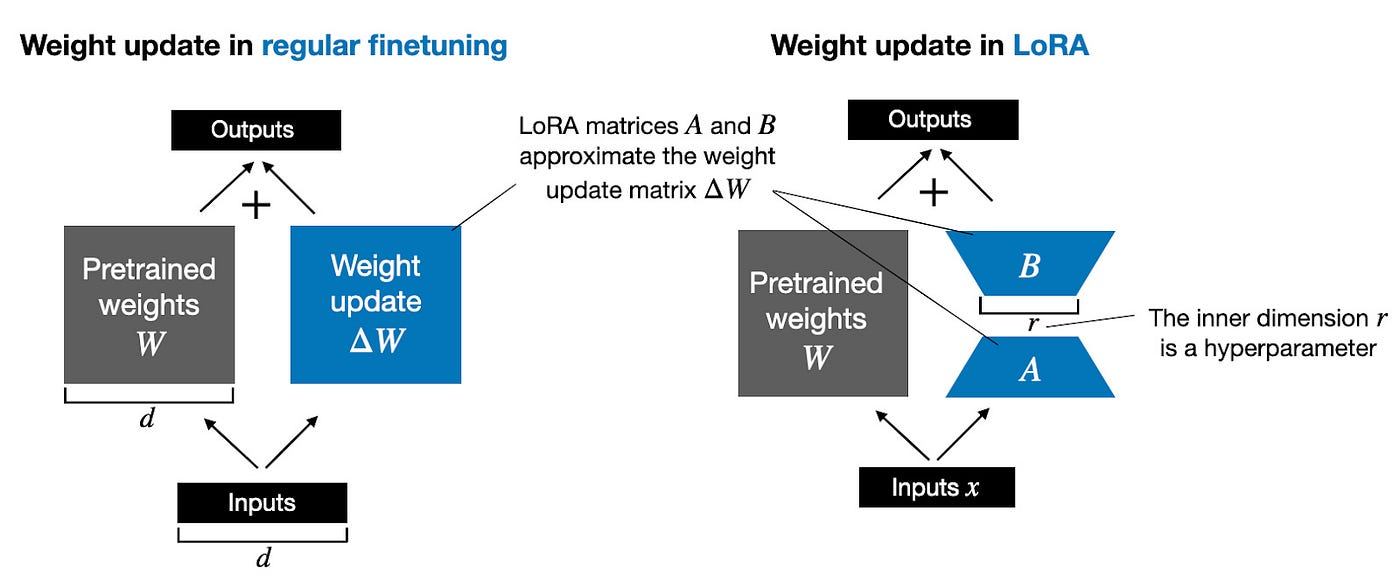
\includegraphics[width=0.75\textwidth]{figures/lora_diagram.jpg}
\caption{LoRA: Low-Rank Adaptation of frozen weight matrices \cite{datadriveninvestor2024lora}}
\label{fig:lora}
\end{figure}

\subsubsection{QLoRA: Quantized Low-Rank Adaptation}

\ac{QLoRA}, introduced by Dettmers et al. \cite{dettmers2023qlora}, extends
\ac{LoRA} by combining it with aggressive model quantization. The pre-trained
model is first quantized to 4-bit precision using a novel data type called
NormalFloat4, which reduces its memory footprint by approximately four times
compared to standard 16-bit representations. The \ac{LoRA} adapters are then
trained in 16-bit precision on top of this quantized base.

This combination makes it possible to fine-tune models with tens of billions
of parameters on a single consumer-grade \ac{GPU}, a capability that was
previously restricted to organizations with access to expensive multi-\ac{GPU}
clusters. \ac{QLoRA} has been shown to match the performance of full 16-bit
fine-tuning on a variety of benchmarks while using a fraction of the hardware
resources \cite{dettmers2023qlora}.

\begin{figure}[H]
\centering
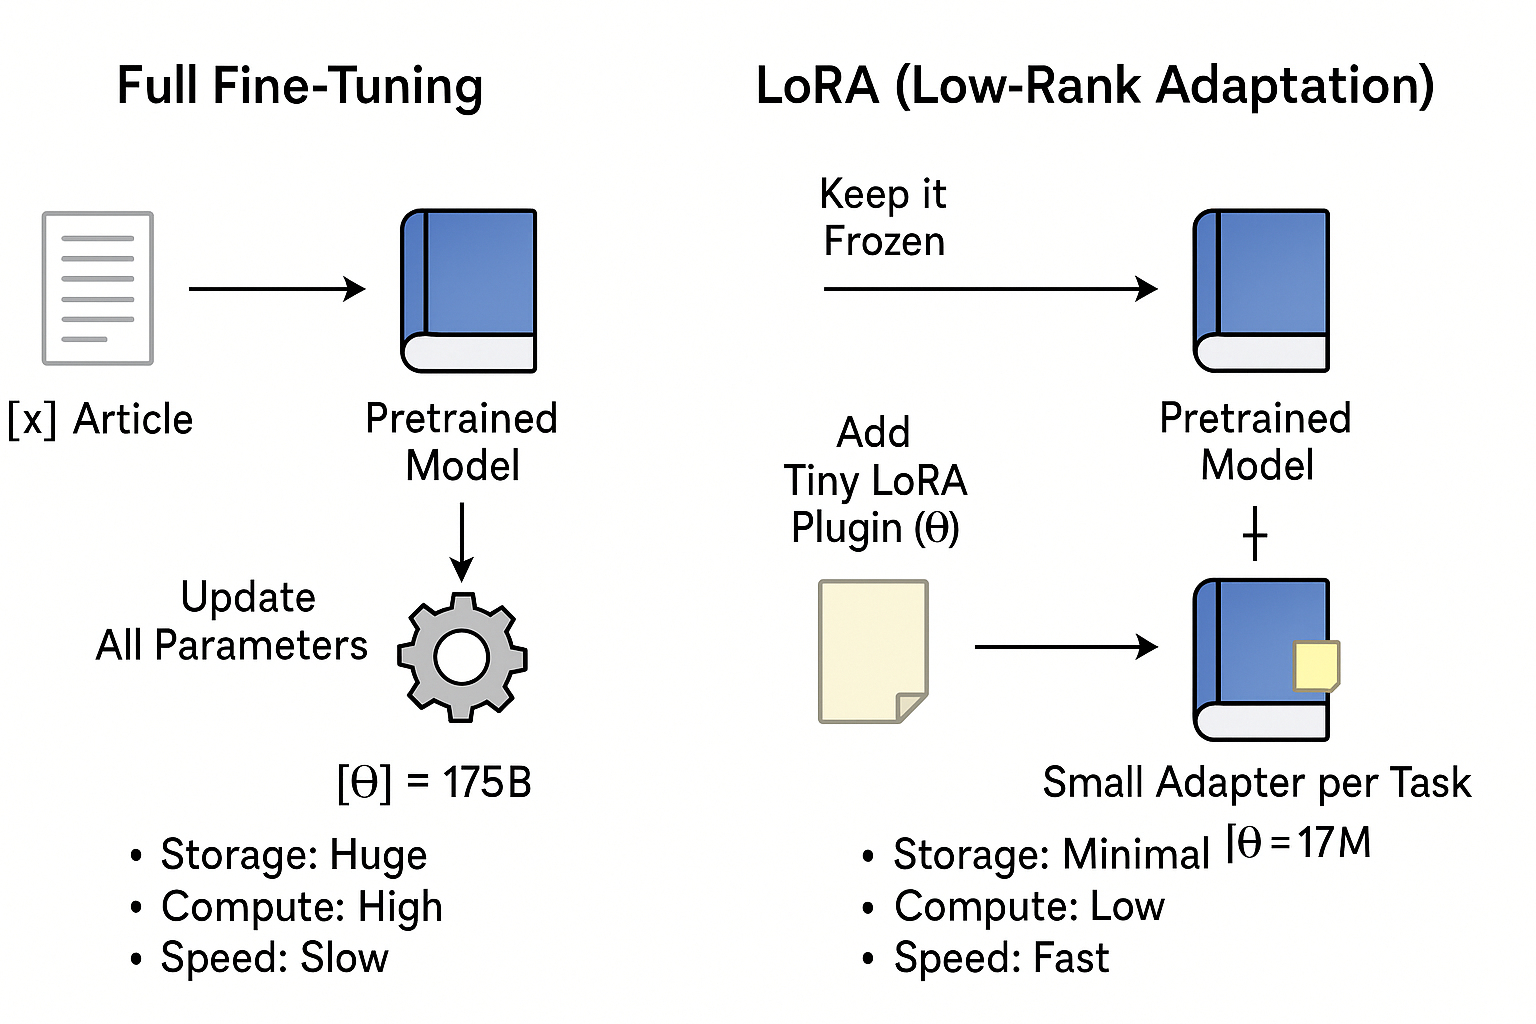
\includegraphics[width=0.7\textwidth]{figures/lora_vs_fft.png}
\caption{LoRA vs Full Fine-Tuning: comparison of parameter update strategies \cite{digitalocean2024lora}}
\label{fig:lora-vs-full}
\end{figure}

\subsection{Domain Adaptation in Specialized Fields}

Fine-tuning for domain adaptation has been successfully applied across a range
of specialized fields, demonstrating that even moderately sized models can
achieve expert-level performance when trained on high-quality domain data:

\begin{itemize}
    \item \textbf{Medical Domain:} Models fine-tuned on clinical notes,
    medical literature, and diagnostic guidelines have shown significant
    improvements in medical question answering and clinical reasoning
    compared to their general-purpose counterparts.

    \item \textbf{Financial Domain:} Language models adapted to financial
    texts (including earnings reports, regulatory filings, and market
    analyses) have demonstrated improved accuracy in sentiment analysis,
    risk assessment, and financial question answering.

    \item \textbf{Legal Domain:} Fine-tuning on legal corpora enables
    models to better understand the hierarchical structure of legislation,
    the precise meaning of legal terminology, and the citation conventions
    that pervade legal reasoning, capabilities that general-purpose models
    consistently lack.
\end{itemize}

These examples validate the approach at the core of our project: fine-tuning
a base model on a curated Tunisian legal corpus to produce a specialized
assistant grounded in the specific vocabulary, structure, and logic of
Tunisian law.

\section{Retrieval-Augmented Generation}
\label{sec:rag}

\subsection{The Hallucination Problem}

Despite their remarkable fluency, \ac{LLM}s are prone to a well-documented
failure mode known as \textbf{hallucination}: the generation of text that
sounds plausible but is factually incorrect, unsupported, or entirely
fabricated. This occurs because language models are fundamentally trained to
produce statistically likely continuations of text, not to verify the factual
accuracy of their outputs \cite{lewis2020rag}.

In high-stakes domains such as law, hallucination is particularly dangerous.
A legal assistant that confidently cites a non-existent article of law or
misrepresents the content of a regulation could mislead users into making
consequential decisions based on false information. Fine-tuning alone cannot
fully eliminate hallucination, because the model's knowledge remains bounded
by its training data and cannot account for legislative updates, newly enacted
regulations, or documents not included in the training corpus.

\subsection{The RAG Paradigm}

\ac{RAG}, first formalized by Lewis et al. \cite{lewis2020rag}, addresses
the hallucination problem by augmenting the language model with an external
knowledge retrieval mechanism. Rather than relying solely on the knowledge
encoded in its parameters, a \ac{RAG}-enabled system retrieves relevant
documents from an external knowledge base at inference time and injects
them into the model's input context before generating a response.

The \ac{RAG} pipeline typically operates in three stages:

\begin{enumerate}
    \item \textbf{Indexing:} Documents from the knowledge base are split into
    manageable chunks, each of which is converted into a dense vector
    representation (embedding) and stored in a vector database.

    \item \textbf{Retrieval:} When a user submits a query, the query is
    similarly converted into an embedding, and the vector database is searched
    for the most semantically similar document chunks using approximate nearest
    neighbor algorithms.

    \item \textbf{Generation:} The retrieved chunks are concatenated with
    the original query and passed to the language model, which generates
    a response grounded in the retrieved evidence.
\end{enumerate}

This architecture enables the system to provide responses that are anchored
in actual documents, significantly reducing hallucination and allowing the
knowledge base to be updated independently of the model itself
\cite{lewis2020rag}.

\begin{figure}[H]
\centering
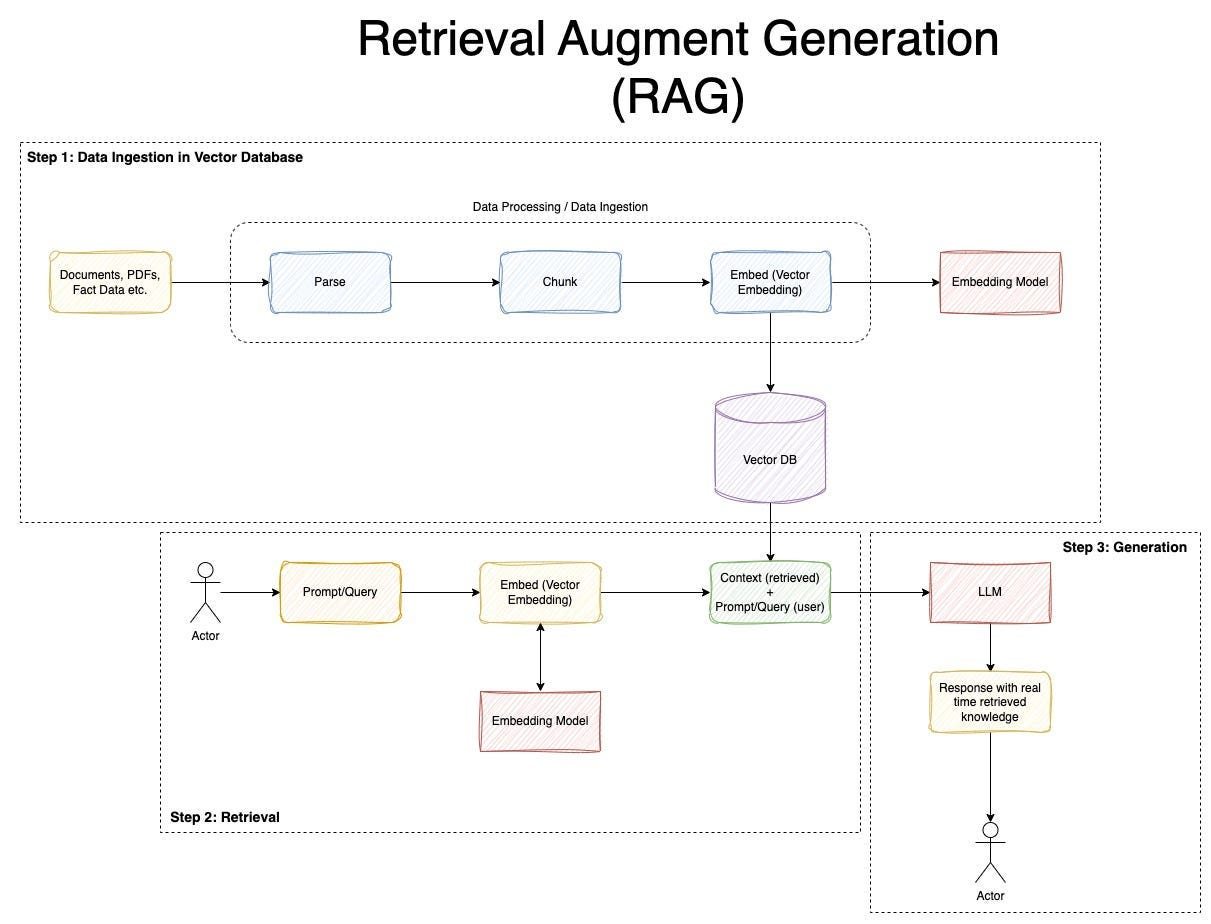
\includegraphics[width=0.9\textwidth]{figures/rag_pipeline.jpg}
\caption{The RAG Pipeline: indexing, retrieval, and generation stages \cite{towardsai2024rag}}
\label{fig:rag-pipeline}
\end{figure}

\subsection{Vector Databases and Embedding Models}

A critical component of any \ac{RAG} pipeline is the \textbf{vector database},
a specialized storage system built to index and search high-dimensional vector
representations at scale. Rather than matching records on exact field values
as relational databases do, vector databases rank results by geometric
proximity, using metrics such as cosine similarity or dot product to surface
the vectors closest to a given query.

\textbf{\ac{FAISS} (Meta).} Developed by Meta Research, \ac{FAISS} is an
open-source library purpose-built for dense vector search over very large
collections. It supports both exact and approximate nearest-neighbor
algorithms, giving practitioners a trade-off between search precision and
speed depending on the scale of their dataset \cite{johnson2019faiss}.

\textbf{Chroma.} Chroma is a lightweight vector store aimed at developers
building \ac{AI} applications. Its straightforward \ac{API} makes it easy
to store, query, and manage embeddings, and it can operate either as an
embedded in-process database or as a standalone server, keeping the
integration overhead low \cite{chroma2024docs}.

\begin{figure}[H]
\centering
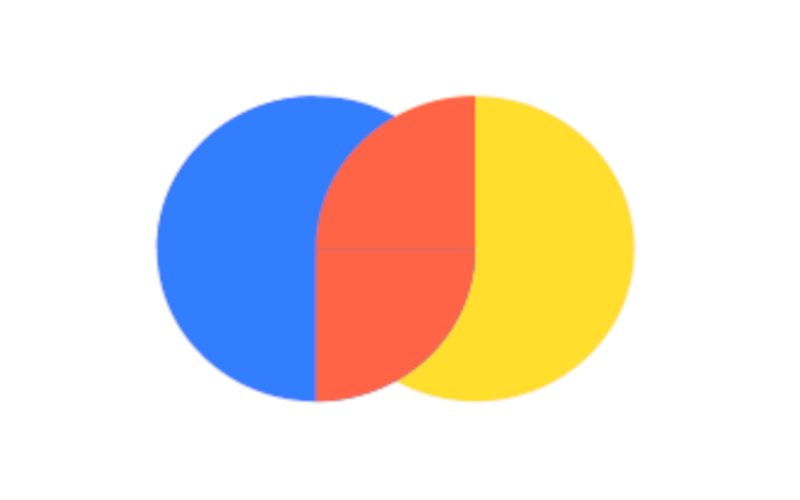
\includegraphics[width=0.18\textwidth]{figures/chroma_logo.png}
\caption{Chroma Vector Database \cite{chroma2024docs}}
\label{fig:chroma-logo}
\end{figure}

\textbf{Qdrant.} Qdrant is a production-grade vector database that goes
beyond basic similarity search by supporting rich payload filtering alongside
vector queries. Its distributed architecture allows it to scale horizontally,
making it suitable for workloads that combine dense retrieval with structured
metadata filtering \cite{qdrant2024docs}.

\begin{figure}[H]
\centering

\includegraphics[width=0.18\textwidth]{figures/qdrant_logo.png}
\caption{Qdrant Vector Database \cite{qdrant2024docs}}
\label{fig:qdrant-logo}
\end{figure}

Retrieval quality depends not only on the vector database but equally on the
\textbf{embedding model} responsible for converting text into vector
representations. The embedding model must map semantically related passages
to nearby points in vector space so that a user query retrieves the most
relevant content even when the phrasing differs from the source document.
Several embedding models are widely used in \ac{RAG} pipelines:

\begin{itemize}
    \item \textbf{Sentence Transformers (SBERT):} A family of models built
    on top of \ac{BERT} and trained specifically to produce sentence-level
    embeddings. They are fast, lightweight, and well suited for monolingual
    or bilingual applications, but their multilingual coverage can be
    limited depending on the variant used \cite{reimers2019sentencebert}.

    \item \textbf{OpenAI text-embedding models:} Proprietary embedding
    models accessible via \ac{API} that deliver strong performance across
    a wide range of languages and tasks. Their main drawback is that they
    require sending data to an external cloud service, which makes them
    incompatible with on-premises deployment requirements.

    \item \textbf{BGE-M3 (BAAI):} Developed by the Beijing Academy of
    Artificial Intelligence, BGE-M3 handles over 100 languages within a
    single model and supports dense, sparse, and multi-vector retrieval 
    simultaneously \cite{chen2024bgem3}. This combination is particularly
    valuable for legal corpora that mix Arabic and French, and where both
    semantic similarity and precise keyword matching are needed.
\end{itemize}

For our project, we selected \textbf{BGE-M3} as the embedding model. Its
native support for Arabic and French within a single unified model, combined
with its ability to run fully on-premises without any external dependency,
makes it the most suitable choice for our Tunisian legal corpus
\cite{chen2024bgem3}.

\subsection{Chunking Strategies}

Before documents can be embedded and indexed, they must be divided into smaller
units called \textbf{chunks}. The choice of chunking strategy directly impacts
retrieval quality:

\begin{itemize}
    \item \textbf{Fixed-size chunking} divides documents into segments of a
    predetermined token or character count. It is simple to implement but
    may split semantically coherent passages across chunk boundaries.

    \item \textbf{Semantic chunking} uses structural cues, such as paragraph
    boundaries, section headings, or sentence boundaries, to create chunks
    that preserve the logical organization of the text.

    \item \textbf{Recursive chunking} attempts to split text at natural
    boundaries (paragraphs first, then sentences, then words) while
    respecting a maximum chunk size, striking a balance between semantic
    coherence and size constraints.
\end{itemize}

For legal documents, where the meaning of a clause or article depends on
its complete text and its position within a hierarchical structure, semantic
or recursive chunking strategies are generally preferred over fixed-size
approaches.

\begin{figure}[H]
\centering
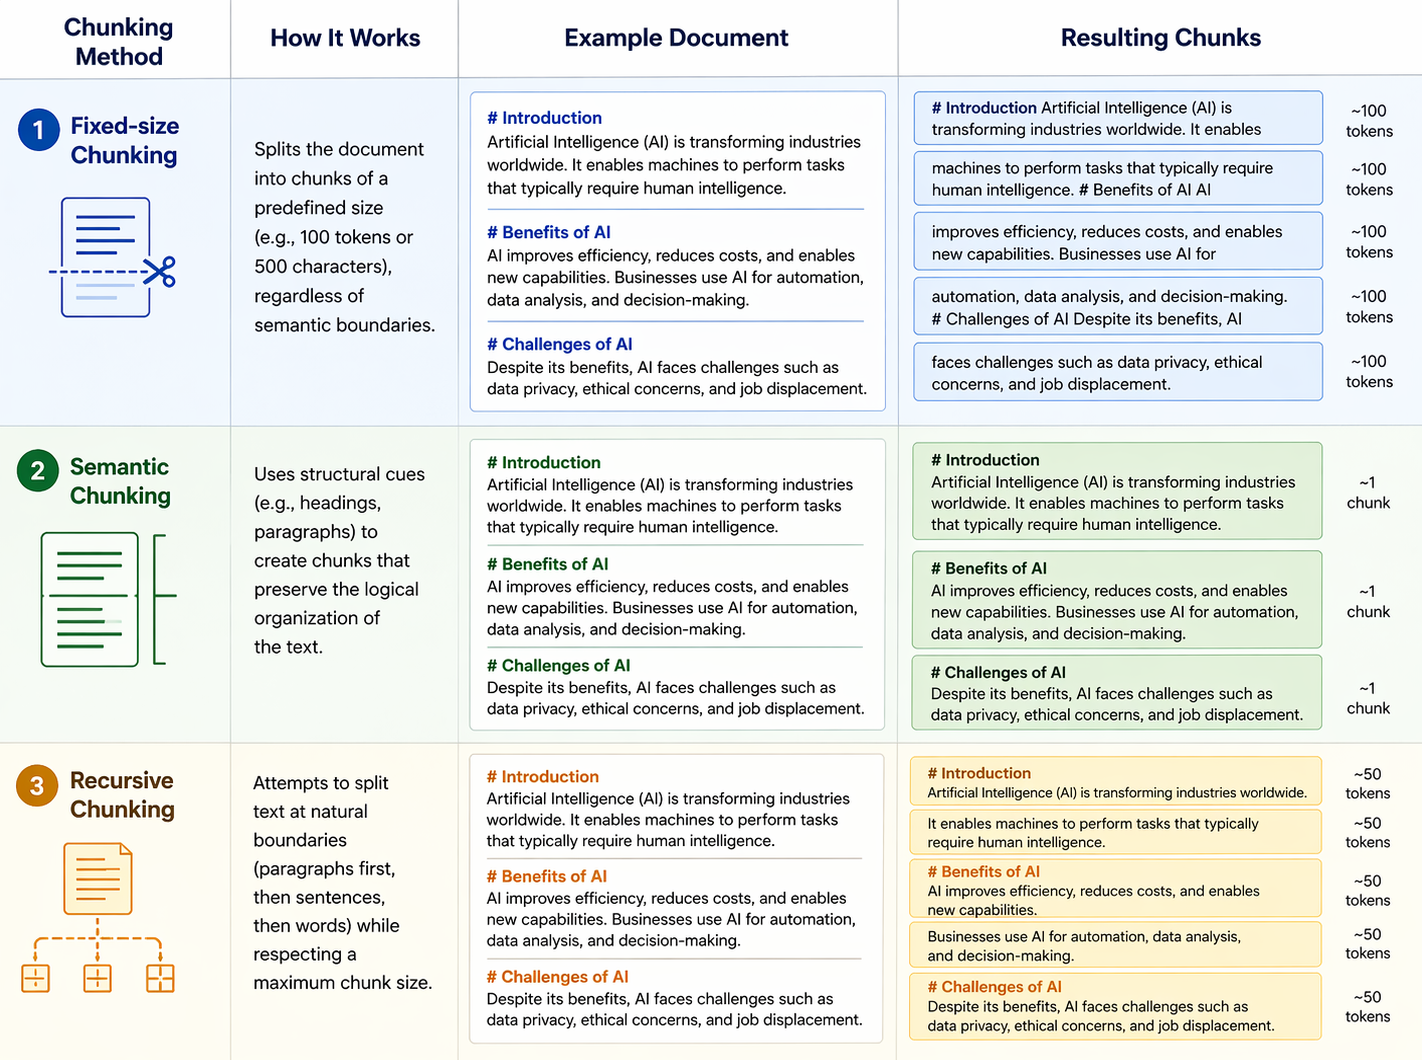
\includegraphics[width=0.9\textwidth]{figures/chunking_methodes.png}
\caption{Overview of Common Chunking Strategies for RAG Pipelines}
\label{fig:chunking-methods}
\end{figure}

\section{AI for Legal Applications}
\label{sec:legal-ai}

\subsection{Challenges Specific to Legal NLP}

Applying \ac{NLP} techniques to legal texts presents a distinct set of
challenges that differ significantly from general-purpose language tasks:

\begin{itemize}
    \item \textbf{Terminological Precision:} Legal language relies on a
    specialized vocabulary where terms carry precise definitions that
    differ from their everyday usage. A model that conflates the legal
    and colloquial meanings of a term may produce misleading outputs.

    \item \textbf{Hierarchical Document Structure:} Legal texts are
    organized in rigid hierarchical structures ( codes, titles, chapters,
    sections, articles, and clauses) that carry semantic significance.
    Understanding a legal provision often requires awareness of its
    position within this hierarchy.

    \item \textbf{Cross-Referencing and Citation:} Legal reasoning is
    deeply referential: articles frequently cite other articles,
    regulations reference enabling legislation, and judicial decisions
    build upon prior rulings. A model must be capable of following
    these reference chains to provide accurate answers.

    \item \textbf{Jurisdictional Specificity:} Legal systems vary
    significantly across jurisdictions. A model trained primarily on
    common law texts will perform poorly on questions about Tunisian
    civil law, as the legal principles, procedural rules, and
    legislative structures are fundamentally different.

    \item \textbf{Multilingual Requirements:} In countries like Tunisia,
    legal documents may exist in multiple languages, primarily Arabic
    and French, and a model must handle both languages to cover the
    full scope of the legal corpus.
\end{itemize}

\subsection{Existing Legal AI Systems Worldwide}

The application of \ac{AI} to legal services has grown rapidly in recent years,
with several notable systems emerging across different jurisdictions:

\begin{itemize}
    \item \textbf{Harvey AI:} A legal \ac{AI} platform built on top of
    OpenAI's models, designed for large law firms. Harvey provides
    contract analysis, legal research assistance, and document drafting
    capabilities, primarily targeting English-speaking common law
    jurisdictions \cite{harvey2024website}.

    \item \textbf{Doctrine.fr:} A French legal intelligence platform that
    uses \ac{AI} to search and analyze French case law, legislation, and
    legal commentary. It provides contextualized search results and
    cross-references across French legal sources \cite{doctrine2024website}.

    \item \textbf{CaseText (now part of Thomson Reuters):} An \ac{AI}-powered
    legal research platform that uses natural language search to help
    lawyers find relevant case law and statutory provisions, primarily
    within the United States legal system \cite{casetext2024website}.

    \item \textbf{Luminance:} A legal \ac{AI} tool focused on contract
    review and due diligence, using machine learning to identify anomalies,
    risks, and key provisions across large volumes of documents \cite{luminance2024website}.
\end{itemize}

\subsection{Arabic and French Legal NLP}

Research on legal \ac{NLP} in Arabic and French remains significantly less
mature than its English counterpart. While a growing body of work has
explored Arabic \ac{NLP} in general domains, including sentiment analysis,
named entity recognition, and machine translation, legal-specific Arabic
\ac{NLP} remains an underexplored area. The challenges are compounded by:

\begin{itemize}
    \item The morphological complexity of Arabic, which makes tokenization
    and entity extraction more difficult than in European languages.

    \item The scarcity of publicly available Arabic legal corpora suitable
    for training or evaluating language models.

    \item The diversity of Arabic dialects and legal terminology across
    different Arab countries, which limits the transferability of models
    trained on one country's legal texts to another.
\end{itemize}

French legal \ac{NLP} benefits from a larger body of digitized legal texts
and more active research communities, but specialized models for Tunisian
law, which operates under a distinct civil code and regulatory framework,
remain virtually nonexistent. This gap is precisely what our project seeks
to address.

\section{On-Premises LLM Deployment}
\label{sec:onpremises}

Deploying \ac{LLM}s on local infrastructure, rather than relying on
cloud-hosted \ac{API}s, introduces a distinct set of technical challenges
that must be addressed to make the system viable within the resource
constraints of an on-premises environment.

\subsection{Model Quantization Techniques}

Running a language model with billions of parameters in its original
precision (typically 16-bit or 32-bit floating point) requires enormous
amounts of \ac{VRAM}. \textbf{Quantization} is the process of reducing
the numerical precision of model weightsm for instance, from 16-bit
to 8-bit or 4-bit, to decrease memory consumption and accelerate
inference, often with minimal impact on output quality.

Two widely adopted quantization formats are:

\begin{itemize}
    \item \textbf{\ac{GGUF}:} A file format designed for efficient local
    inference, particularly on \ac{CPU}-based systems. \ac{GGUF} supports
    a range of quantization levels (from 2-bit to 8-bit) and is the
    native format used by llama.cpp and Ollama for loading and running
    models locally \cite{ollama2024docs}.

    \item \textbf{\ac{GPTQ}:} A post-training quantization method that
    compresses model weights to 4-bit or 3-bit precision while minimizing
    the loss in output quality. \ac{GPTQ} is optimized for \ac{GPU}-based
    inference and is widely supported by inference frameworks such as
    vLLM and text-generation-inference \cite{frantar2022gptq}.
\end{itemize}

\subsection{Local Inference Frameworks}

Several frameworks have been developed to facilitate the deployment and
execution of \ac{LLM}s on local hardware.

\textbf{Ollama.} An open-source tool that simplifies the process of
downloading, running, and managing \ac{LLM}s on local machines. Ollama
provides a command-line interface and a local \ac{API} server, supports
\ac{GGUF}-quantized models, and handles model lifecycle management
(downloading, loading, and unloading) automatically. It is the inference
framework selected for our project's on-premises deployment at \ac{ATI}
Tunisie \cite{ollama2024docs}.

\begin{figure}[H]
\centering

\includegraphics[width=0.25\textwidth]{figures/ollama_logo.png}
\caption{Ollama Local Inference Framework \cite{ollama2024docs}}
\label{fig:ollama-logo}
\end{figure}

\textbf{vLLM.} A high-throughput inference engine designed for
production-grade \ac{LLM} serving. vLLM introduces PagedAttention,
a memory management technique that significantly improves \ac{GPU}
memory utilization during inference, enabling higher concurrent
request throughput than traditional serving approaches
\cite{kwon2023vllm}.

\begin{figure}[H]
\centering

\includegraphics[width=0.25\textwidth]{figures/vllm_logo.png}
\caption{vLLM Inference Engine \cite{kwon2023vllm}}
\label{fig:vllm-logo}
\end{figure}

\textbf{llama.cpp.} A lightweight C/C++ inference library focused on
running \ac{LLM}s efficiently on \ac{CPU} hardware. It supports a wide
range of quantization formats and is the engine underlying Ollama's
model execution \cite{ollama2024docs}.

\begin{figure}[H]
\centering

\includegraphics[width=0.25\textwidth]{figures/llamacpp_logo.png}
\caption{llama.cpp Inference Library \cite{ollama2024docs}}
\label{fig:llamacpp-logo}
\end{figure}

\subsection{Hardware Constraints and Optimization}

On-premises deployment imposes strict hardware constraints that influence
every architectural decision. Unlike cloud environments where resources
can be scaled elastically, a local deployment must operate within fixed
\ac{RAM}, \ac{VRAM}, and compute budgets. Key considerations include:

\begin{itemize}
    \item \textbf{Model Size vs. Quality Trade-off:} Smaller quantized
    models run faster and require less memory, but may sacrifice output
    quality. The choice of model size and quantization level must balance
    response quality against the available hardware resources.

    \item \textbf{Inference Latency:} Users expect near-instantaneous
    responses from a conversational assistant. Model quantization and
    efficient batching strategies help reduce the time between receiving
    a query and producing the first output token.

    \item \textbf{Concurrent Users:} The system must be capable of serving
    multiple users simultaneously without degrading response times. This
    requires careful memory management and potentially request queuing
    mechanisms.
\end{itemize}

\section{Comparative Study of Existing Legal AI Solutions}
\label{sec:comparative-study}

To position our project within the broader landscape of legal \ac{AI},
Table~\ref{tab:legal-ai-comparison} presents a structured comparison of
existing solutions against the specific requirements identified in our
problem statement.

\begin{table}[H]
\centering
\caption{Comparative Analysis of Existing Legal AI Solutions}
\label{tab:legal-ai-comparison}
\renewcommand{\arraystretch}{1.3}
\begin{tabular}{|p{2.5cm}|p{2cm}|p{2cm}|p{2cm}|p{2cm}|p{2cm}|}
\hline
\textbf{Criteria} & \textbf{Harvey AI} & \textbf{Doctrine.fr} & \textbf{CaseText} & \textbf{Luminance} & \textbf{Our Solution} \\
\hline
Target Jurisdiction &
Common Law (US/UK) &
French Law &
US Law &
Multi-jurisdiction &
Tunisian Law \\
\hline
Tunisian Legal Knowledge &
None &
None &
None &
None &
Fine-tuned on Tunisian corpus \\
\hline
Language Support &
English &
French &
English &
English &
Arabic \& French \\
\hline
Deployment Model &
Cloud-only &
Cloud-only &
Cloud-only &
Cloud-only &
On-premises \\
\hline
Data Sovereignty &
No &
No &
No &
No &
Full \\
\hline
Knowledge Update Mechanism &
Periodic retraining &
Database updates &
Database updates &
Periodic retraining &
\ac{RAG} pipeline \\
\hline
Domain Adaptation Method &
Prompt engineering &
Custom search engine &
Prompt engineering &
Proprietary \ac{AI} &
Fine-tuned \ac{LLM} + \ac{RAG} \\
\hline
Open Source &
No &
No &
No &
No &
Yes \\
\hline
\end{tabular}
\end{table}

The comparative analysis reveals that no existing solution addresses the
combination of requirements central to our project: deep specialization in
Tunisian law, support for both Arabic and French, full on-premises deployment
with data sovereignty guarantees, and a hybrid fine-tuning plus \ac{RAG}
approach for domain adaptation. Each existing platform is either jurisdiction-locked
to a foreign legal system, dependent on cloud infrastructure, or both. This
gap validates the need for the specialized system proposed in Chapter~I and
provides a clear positioning for our contribution.

\section{Functional and Non-Functional Requirements}
\label{sec:requirements}

Before proceeding to the design and implementation of our solution, it is
essential to formalize the requirements that the system must satisfy. These
requirements are derived from the problem analysis conducted in Chapter~I,
the technical constraints identified in the preceding sections, and the
operational needs expressed by E-Tafakna and \ac{ATI} Tunisie.

\subsection{Functional Requirements}

Functional requirements define what the system must be able to do, the
concrete capabilities it must provide to its users and to the broader
platform it integrates with.

\begin{table}[H]
\centering
\caption{Functional Requirements}
\label{tab:functional-requirements}
\renewcommand{\arraystretch}{1.5}
\begin{tabular}{|p{1cm}|p{4cm}|p{8.5cm}|}
\hline
\textbf{ID} & \textbf{Requirement} & \textbf{Description} \\
\hline
RF01 & Legal Question Answering &
The system must be able to receive a legal question in Arabic or French
and produce an accurate, contextually relevant answer grounded in Tunisian
legislation. \\
\hline
RF02 & Document-Grounded Responses &
Each response must be supported by specific legal texts retrieved from the
knowledge base. The system must cite the source documents (law number,
article, decree) used to generate its answer. \\
\hline
RF03 & Corpus Ingestion and Indexing &
The system must provide a mechanism to ingest new legal documents (in
\ac{PDF} or text format), process them, and add them to the vector
database for future retrieval. \\
\hline
RF04 & Bilingual Support &
The system must handle queries and produce responses in both Arabic and
French, reflecting the bilingual nature of the Tunisian legal corpus. \\
\hline
RF05 & Conversational Interface &
The system must expose a conversational interface (via \ac{API}) that
allows natural language interaction, maintaining context across multiple
turns within a session. \\
\hline
RF06 & Platform Integration &
The system must provide \ac{API} endpoints compatible with E-Tafakna's
existing platform, enabling integration with both Elyssa and Kahina
without requiring changes to the user-facing interface. \\
\hline
RF07 & Knowledge Base Update &
The system must support the addition of new legal documents to the
knowledge base without requiring model retraining, ensuring that
legislative updates can be incorporated dynamically through the
\ac{RAG} pipeline. \\
\hline
\end{tabular}
\end{table}

\subsection{Non-Functional Requirements}

Non-functional requirements define the quality attributes that the system
must exhibit, constraints on how it performs its functions rather than
what functions it provides.

\begin{table}[H]
\centering
\caption{Non-Functional Requirements}
\label{tab:non-functional-requirements}
\renewcommand{\arraystretch}{1.5}
\begin{tabular}{|p{1.2cm}|p{4cm}|p{8.5cm}|}
\hline
\textbf{ID} & \textbf{Requirement} & \textbf{Description} \\
\hline
RNF01 & On-Premises Deployment &
The entire system (language model, \ac{RAG} pipeline, and vector
database) must run on \ac{ATI} Tunisie's local infrastructure with
no dependency on external cloud services or \ac{API}s. \\
\hline
RNF02 & Data Sovereignty &
All legal data processed by the system must remain within \ac{ATI}
Tunisie's secure environment. No data may be transmitted to external
servers at any stage of processing or inference. \\
\hline
RNF03 & Response Latency &
The system must generate a complete response within a reasonable
time frame (target: under 30 seconds for a typical legal query),
ensuring a fluid conversational experience for end users. \\
\hline
RNF04 & Legal Accuracy &
Responses must demonstrate a measurably higher accuracy on Tunisian
legal questions compared to a generic, non-fine-tuned baseline model,
as validated through the evaluation protocol defined in the \ac{DSR}
methodology. \\
\hline
RNF05 & Scalability &
The system architecture must support serving multiple concurrent
users without significant degradation of response quality or latency. \\
\hline
RNF06 & Maintainability &
The system must be designed with clear separation of concerns
(model serving, retrieval pipeline, and \ac{API} layer) to facilitate
future maintenance, updates, and component-level improvements. \\
\hline
RNF07 & Security &
Access to the system's \ac{API} endpoints must be secured through
authentication mechanisms, and all communication between components
must occur within the local network perimeter. \\
\hline
\end{tabular}
\end{table}

\section{Conclusion}

This chapter provided a comprehensive review of the technological foundations
and the current state of research underpinning our project. We examined the
architecture and capabilities of modern \ac{LLM}s, explored fine-tuning
techniques, from full fine-tuning to parameter-efficient methods such as
\ac{LoRA} and \ac{QLoRA}, and detailed the \ac{RAG} paradigm as a solution
to the hallucination problem inherent in language models.

We then surveyed the specific challenges of applying \ac{NLP} to legal texts,
reviewed existing legal \ac{AI} solutions across different jurisdictions, and
confirmed that none addresses the unique combination of requirements central
to our project: deep specialization in Tunisian law, bilingual Arabic-French
support, and fully on-premises deployment with data sovereignty guarantees.
The technical challenges of local \ac{LLM} deployment, including model
quantization and inference framework selection, were also examined.

Finally, we formalized the functional and non-functional requirements that
will guide the design and implementation of our system, providing a clear
specification against which the final artifact can be evaluated.

The following chapter will present the detailed design and architecture of
our solution, translating these requirements into concrete technical choices
and system components.
